\subsection{Session 2, Exercise 5}

\lineparagraph{Exercise}

Which words are accepted by this automaton? ($\Sigma=\{0,1\}$).

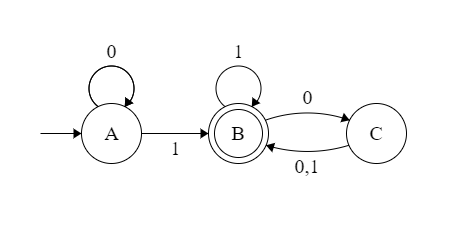
\includegraphics[width=0.5\linewidth]{02/2_5_automaton.png}

\lineparagraph{Solution}

I want to prove that the states mean the following in the given automaton:

\begin{itemize}
    \item State $A$: words that don't contain a $1$.
    \item State $B$: words that contain a $1$ and end in an even number of $0$'s (including zero number of $0$'s).
    \item State $C$: words that contain a $1$ and end in an odd number of $0$'s.
\end{itemize}

We can look at the defined transitions to prove that this is indeed correct:

\begin{itemize}
    \item In state $A$ as long as we only read $0$'s in, we stay in state $A$. If we read a single $1$ in, we move away and we can never come back. So only words that contain no $1$'s can end up in state $A$.
    \item In state $B$ and $C$ the word already contains a $1$, since we left $A$.
    \item If we read in a $1$ in either $B$ or $C$ we always ''reset'' to $B$ back: since when the input ends in a $1$, that means that it ends in an even (zero) number of $0$'s. This is done by the transitions $B\xrightarrow{1}B$ and $C\xrightarrow{1}B$.
    \item If we read a $0$ in state $B$ the parity of the ending zeroes changes from even to odd, and vice versa for state $C$. These are done by the transitions $B\xrightarrow{0}C$ and $C\xrightarrow{0}B$.
\end{itemize}

Furthermore the starting state is correct:
\begin{itemize}
    \item The starting state is state $A$, since the empty string contains no $1$'s, which is represented by state $A$.
\end{itemize}

Now let's look at the accepting/rejecting states:

\begin{itemize}
    \item State $B$ accepts, which means that the language of the automaton is \textbf{''words that contain a $1$ and end in an even number of $0$'s (including zero number of $0$'s)''}.
    \item The other two states $A$ and $C$ reject (which means words that don't contain a $1$ and words that contain a $1$ but end in an odd number of $0$'s are rejected).
\end{itemize}